\documentclass[11pt]{article}
% Course template settings (Essentials in Text and Speech Processing, UZH): 11pt, A4, 2cm/3cm margins.
\usepackage[english]{babel}
\usepackage[a4paper,top=2cm,bottom=2cm,left=3cm,right=3cm,marginparwidth=1.75cm]{geometry}
\usepackage[T1]{fontenc}
\usepackage[utf8]{inputenc}
\usepackage{mathptmx}
\usepackage{courier}
\usepackage{newunicodechar}
\newunicodechar{ā}{\=a}\newunicodechar{ē}{\=e}\newunicodechar{ī}{\={\i}}\newunicodechar{ō}{\=o}
\newunicodechar{ū}{\=u}\newunicodechar{ȳ}{\=y}\newunicodechar{ǣ}{\=\ae}\newunicodechar{Ā}{\=A}
\newunicodechar{Ē}{\=E}\newunicodechar{Ō}{\=O}\newunicodechar{Ū}{\=U}\newunicodechar{Ǣ}{\=\AE}
\newunicodechar{ô}{\^o}\newunicodechar{â}{\^a}\newunicodechar{±}{\ensuremath{\pm}}
\usepackage{amsmath}
\usepackage{graphicx}
\usepackage{booktabs}
\usepackage[font=normalsize,labelfont=bf]{caption}
\usepackage[colorlinks=true,allcolors=blue]{hyperref}
\usepackage{xurl}
\setlength{\tabcolsep}{4.5pt}
\setlength{\emergencystretch}{2em}
% abstract at full 11pt (the article default sets it, and its heading, in \small)
\renewenvironment{abstract}{\begin{center}\textbf{Abstract}\end{center}\begin{quotation}\noindent\ignorespaces}{\end{quotation}}
% generated by src/oevl/build_report.py from data/ and results/ -- do not edit
\newcommand{\NABeoAFB}{132}
\newcommand{\NABeoAFL}{132}
\newcommand{\NABeoAFW}{118}
\newcommand{\NABeoALB}{31}
\newcommand{\NABeoAWB}{57}
\newcommand{\NABeoAWL}{54}
\newcommand{\NABeoAllBil}{91.69}
\newcommand{\NABeoAllFreq}{92.39}
\newcommand{\NABeoAllLeft}{91.69}
\newcommand{\NABeoAllN}{17,361}
\newcommand{\NABeoAllOrc}{96.14}
\newcommand{\NABeoAllWord}{91.70}
\newcommand{\NABeoAttBil}{90.65}
\newcommand{\NABeoAttFreq}{90.67}
\newcommand{\NABeoAttLeft}{90.75}
\newcommand{\NABeoAttN}{3,268}
\newcommand{\NABeoAttOrc}{100.00}
\newcommand{\NABeoAttWord}{90.62}
\newcommand{\NABeoBFB}{255}
\newcommand{\NABeoBFL}{254}
\newcommand{\NABeoBFW}{242}
\newcommand{\NABeoBLB}{32}
\newcommand{\NABeoBWB}{56}
\newcommand{\NABeoBWL}{52}
\newcommand{\NABeoLexBil}{87.07}
\newcommand{\NABeoLexFreq}{89.10}
\newcommand{\NABeoLexLeft}{87.08}
\newcommand{\NABeoLexN}{6,007}
\newcommand{\NABeoLexOrc}{99.93}
\newcommand{\NABeoLexWord}{87.09}
\newcommand{\NABeoMinBil}{5.33}
\newcommand{\NABeoMinFreq}{0.00}
\newcommand{\NABeoMinLeft}{6.15}
\newcommand{\NABeoMinN}{325}
\newcommand{\NABeoMinOrc}{100.00}
\newcommand{\NABeoMinP}{5.9e-11}
\newcommand{\NABeoMinWord}{1.54}
\newcommand{\NABeoPFB}{4.0e-10}
\newcommand{\NABeoPFL}{5.3e-10}
\newcommand{\NABeoPFW}{5.9e-11}
\newcommand{\NABeoPLB}{1.0000}
\newcommand{\NABeoPWB}{1.0000}
\newcommand{\NABeoPWL}{0.9227}
\newcommand{\NASolAFB}{202}
\newcommand{\NASolAFL}{194}
\newcommand{\NASolAFW}{137}
\newcommand{\NASolALB}{44}
\newcommand{\NASolAWB}{102}
\newcommand{\NASolAWL}{86}
\newcommand{\NASolAllBil}{89.82}
\newcommand{\NASolAllFreq}{89.29}
\newcommand{\NASolAllLeft}{89.84}
\newcommand{\NASolAllN}{15,426}
\newcommand{\NASolAllOrc}{95.07}
\newcommand{\NASolAllWord}{89.53}
\newcommand{\NASolAttBil}{88.41}
\newcommand{\NASolAttFreq}{87.39}
\newcommand{\NASolAttLeft}{88.62}
\newcommand{\NASolAttN}{4,497}
\newcommand{\NASolAttOrc}{100.00}
\newcommand{\NASolAttWord}{87.59}
\newcommand{\NASolBFB}{122}
\newcommand{\NASolBFL}{102}
\newcommand{\NASolBFW}{111}
\newcommand{\NASolBLB}{56}
\newcommand{\NASolBWB}{48}
\newcommand{\NASolBWL}{20}
\newcommand{\NASolLexBil}{89.06}
\newcommand{\NASolLexFreq}{88.00}
\newcommand{\NASolLexLeft}{89.11}
\newcommand{\NASolLexN}{7,597}
\newcommand{\NASolLexOrc}{99.74}
\newcommand{\NASolLexWord}{88.49}
\newcommand{\NASolMinBil}{10.65}
\newcommand{\NASolMinFreq}{0.00}
\newcommand{\NASolMinLeft}{10.32}
\newcommand{\NASolMinN}{604}
\newcommand{\NASolMinOrc}{100.00}
\newcommand{\NASolMinP}{9.8e-08}
\newcommand{\NASolMinWord}{2.48}
\newcommand{\NASolPFB}{1.0e-05}
\newcommand{\NASolPFL}{9.8e-08}
\newcommand{\NASolPFW}{0.1122}
\newcommand{\NASolPLB}{0.2713}
\newcommand{\NASolPWB}{1.2e-05}
\newcommand{\NASolPWL}{6.2e-11}
\newcommand{\NBeoGain}{7.14}
\newcommand{\NBeoGainBil}{7.05}
\newcommand{\NBeoGainDict}{10.13}
\newcommand{\NBeoGainDictWiki}{3.00}
\newcommand{\NBeoGainLeft}{7.05}
\newcommand{\NBeoGainWord}{7.17}
\newcommand{\NBeoNoCandTrue}{32.4}
\newcommand{\NBeoTokens}{17,361}
\newcommand{\NBeoUnknown}{31.5}
\newcommand{\NBootBeoClsBBilVsFreq}{+2.14}
\newcommand{\NBootBeoClsBBilVsFreqHi}{+3.81}
\newcommand{\NBootBeoClsBBilVsFreqLo}{+0.47}
\newcommand{\NBootBeoClsBBilVsLeft}{-1.59}
\newcommand{\NBootBeoClsBBilVsLeftHi}{-0.33}
\newcommand{\NBootBeoClsBBilVsLeftLo}{-2.97}
\newcommand{\NBootBeoClsBBilVsWord}{+2.14}
\newcommand{\NBootBeoClsBBilVsWordHi}{+3.81}
\newcommand{\NBootBeoClsBBilVsWordLo}{+0.47}
\newcommand{\NBootBeoClsBLeftVsFreq}{+3.73}
\newcommand{\NBootBeoClsBLeftVsFreqHi}{+5.41}
\newcommand{\NBootBeoClsBLeftVsFreqLo}{+2.16}
\newcommand{\NBootBeoClsBLeftVsWord}{+3.73}
\newcommand{\NBootBeoClsBLeftVsWordHi}{+5.41}
\newcommand{\NBootBeoClsBLeftVsWordLo}{+2.16}
\newcommand{\NBootBeoClsBWordVsFreq}{+0.00}
\newcommand{\NBootBeoClsBWordVsFreqHi}{+0.00}
\newcommand{\NBootBeoClsBWordVsFreqLo}{+0.00}
\newcommand{\NBootBeoLexBilVsFreq}{-0.16}
\newcommand{\NBootBeoLexBilVsFreqHi}{+0.35}
\newcommand{\NBootBeoLexBilVsFreqLo}{-0.58}
\newcommand{\NBootBeoLexBilVsLeft}{-0.19}
\newcommand{\NBootBeoLexBilVsLeftHi}{+0.06}
\newcommand{\NBootBeoLexBilVsLeftLo}{-0.43}
\newcommand{\NBootBeoLexBilVsWord}{-0.47}
\newcommand{\NBootBeoLexBilVsWordHi}{-0.13}
\newcommand{\NBootBeoLexBilVsWordLo}{-0.79}
\newcommand{\NBootBeoLexLeftVsFreq}{+0.03}
\newcommand{\NBootBeoLexLeftVsFreqHi}{+0.52}
\newcommand{\NBootBeoLexLeftVsFreqLo}{-0.41}
\newcommand{\NBootBeoLexLeftVsWord}{-0.28}
\newcommand{\NBootBeoLexLeftVsWordHi}{+0.05}
\newcommand{\NBootBeoLexLeftVsWordLo}{-0.63}
\newcommand{\NBootBeoLexWordVsFreq}{+0.31}
\newcommand{\NBootBeoLexWordVsFreqHi}{+0.74}
\newcommand{\NBootBeoLexWordVsFreqLo}{-0.08}
\newcommand{\NBootSolClsBBilVsFreq}{+4.99}
\newcommand{\NBootSolClsBBilVsFreqHi}{+6.36}
\newcommand{\NBootSolClsBBilVsFreqLo}{+3.58}
\newcommand{\NBootSolClsBBilVsLeft}{-0.23}
\newcommand{\NBootSolClsBBilVsLeftHi}{+0.81}
\newcommand{\NBootSolClsBBilVsLeftLo}{-1.23}
\newcommand{\NBootSolClsBBilVsWord}{+4.99}
\newcommand{\NBootSolClsBBilVsWordHi}{+6.36}
\newcommand{\NBootSolClsBBilVsWordLo}{+3.58}
\newcommand{\NBootSolClsBLeftVsFreq}{+5.21}
\newcommand{\NBootSolClsBLeftVsFreqHi}{+6.58}
\newcommand{\NBootSolClsBLeftVsFreqLo}{+3.74}
\newcommand{\NBootSolClsBLeftVsWord}{+5.21}
\newcommand{\NBootSolClsBLeftVsWordHi}{+6.58}
\newcommand{\NBootSolClsBLeftVsWordLo}{+3.74}
\newcommand{\NBootSolClsBWordVsFreq}{+0.00}
\newcommand{\NBootSolClsBWordVsFreqHi}{+0.00}
\newcommand{\NBootSolClsBWordVsFreqLo}{+0.00}
\newcommand{\NBootSolLexBilVsFreq}{+1.21}
\newcommand{\NBootSolLexBilVsFreqHi}{+1.62}
\newcommand{\NBootSolLexBilVsFreqLo}{+0.81}
\newcommand{\NBootSolLexBilVsLeft}{-0.16}
\newcommand{\NBootSolLexBilVsLeftHi}{+0.06}
\newcommand{\NBootSolLexBilVsLeftLo}{-0.40}
\newcommand{\NBootSolLexBilVsWord}{+0.76}
\newcommand{\NBootSolLexBilVsWordHi}{+1.08}
\newcommand{\NBootSolLexBilVsWordLo}{+0.46}
\newcommand{\NBootSolLexLeftVsFreq}{+1.37}
\newcommand{\NBootSolLexLeftVsFreqHi}{+1.75}
\newcommand{\NBootSolLexLeftVsFreqLo}{+1.00}
\newcommand{\NBootSolLexLeftVsWord}{+0.92}
\newcommand{\NBootSolLexLeftVsWordHi}{+1.21}
\newcommand{\NBootSolLexLeftVsWordLo}{+0.64}
\newcommand{\NBootSolLexWordVsFreq}{+0.45}
\newcommand{\NBootSolLexWordVsFreqHi}{+0.70}
\newcommand{\NBootSolLexWordVsFreqLo}{+0.20}
\newcommand{\NCharsiuBeoAll}{77.78}
\newcommand{\NCharsiuBeoLex}{77.10}
\newcommand{\NCharsiuLenOnly}{71}
\newcommand{\NCharsiuLenShare}{75.5}
\newcommand{\NCharsiuN}{500}
\newcommand{\NCharsiuPer}{0.0410}
\newcommand{\NCharsiuSolAll}{70.96}
\newcommand{\NCharsiuSolLex}{72.92}
\newcommand{\NCharsiuSolLexBilFix}{1,362}
\newcommand{\NCharsiuSolLexWordFix}{1,372}
\newcommand{\NCharsiuSolLexWordFixShare}{86.84}
\newcommand{\NCharsiuSolLexWrong}{1,580}
\newcommand{\NCharsiuTrunc}{12}
\newcommand{\NCharsiuWer}{0.208}
\newcommand{\NCharsiuWerFixed}{0.188}
\newcommand{\NCharsiuWordErrors}{94}
\newcommand{\NCheckAlign}{0}
\newcommand{\NCheckEditorial}{54}
\newcommand{\NCheckN}{100}
\newcommand{\NCheckNorm}{10}
\newcommand{\NCheckOther}{36}
\newcommand{\NClassA}{13}
\newcommand{\NClassAgree}{96.67}
\newcommand{\NClassB}{5}
\newcommand{\NClassC}{42}
\newcommand{\NClassKappa}{0.927}
\newcommand{\NCollapseDevLex}{55.94}
\newcommand{\NCollapseDevMostLong}{98.21}
\newcommand{\NCollapseEpochs}{3}
\newcommand{\NCollapseSolAll}{74.10}
\newcommand{\NCollapseSolLex}{52.11}
\newcommand{\NCorpusTokens}{161,062}
\newcommand{\NDThreeSolAllCost}{0.88}
\newcommand{\NDevBilNoZup}{95.31}
\newcommand{\NDevBilZup}{94.41}
\newcommand{\NDevBilZupShared}{94.70}
\newcommand{\NDevFreqNoZup}{95.60}
\newcommand{\NDevFreqZup}{94.87}
\newcommand{\NDevFreqZupShared}{95.12}
\newcommand{\NDevLexShared}{7,639}
\newcommand{\NDevTokens}{16,649}
\newcommand{\NEncBestCtxGainBeo}{0.36}
\newcommand{\NEncBestCtxGainSol}{1.32}
\newcommand{\NEncFullCap}{2,560}
\newcommand{\NEncTrainExamples}{25,949}
\newcommand{\NEncWordGainBeo}{0.29}
\newcommand{\NEncWordGainSol}{0.16}
\newcommand{\NErrCharsiuCeiling}{0}
\newcommand{\NErrCharsiuEditorial}{67}
\newcommand{\NErrCharsiuGoldInDoubt}{5}
\newcommand{\NErrCharsiuGrammatical}{73}
\newcommand{\NErrCharsiuHomograph}{55}
\newcommand{\NErrCharsiuOther}{0}
\newcommand{\NErrCharsiuSegment}{0}
\newcommand{\NErrCharsiuTruncation}{0}
\newcommand{\NErrEncCeiling}{3}
\newcommand{\NErrEncEditorial}{55}
\newcommand{\NErrEncGoldInDoubt}{12}
\newcommand{\NErrEncGrammatical}{73}
\newcommand{\NErrEncHomograph}{57}
\newcommand{\NErrEncOther}{0}
\newcommand{\NErrEncSegment}{0}
\newcommand{\NErrEncTruncation}{0}
\newcommand{\NErrItems}{200}
\newcommand{\NErrKappa}{0.975}
\newcommand{\NGateHTHs}{10.20}
\newcommand{\NGateHTHsFloor}{88.62}
\newcommand{\NGateHTTauber}{9.85}
\newcommand{\NGateHTTauberFloor}{88.97}
\newcommand{\NGateHWHs}{7.45}
\newcommand{\NGateHWHsFloor}{88.63}
\newcommand{\NGateHWWyatt}{6.93}
\newcommand{\NGateHWWyattFloor}{89.15}
\newcommand{\NGateWTTauber}{7.20}
\newcommand{\NGateWTTauberFloor}{88.88}
\newcommand{\NGateWTWyatt}{6.94}
\newcommand{\NGateWTWyattFloor}{89.13}
\newcommand{\NGeMat}{2/252}
\newcommand{\NGeSol}{61/3}
\newcommand{\NGeZup}{0/128}
\newcommand{\NGridCollapsed}{0}
\newcommand{\NGridRuns}{39}
\newcommand{\NLeakDevSent}{34}
\newcommand{\NLeakDevTok}{661}
\newcommand{\NLeakSolSent}{1}
\newcommand{\NLeakSolTok}{49}
\newcommand{\NPBeoAFB}{172}
\newcommand{\NPBeoAFL}{174}
\newcommand{\NPBeoAFW}{153}
\newcommand{\NPBeoALB}{28}
\newcommand{\NPBeoAWB}{60}
\newcommand{\NPBeoAWL}{55}
\newcommand{\NPBeoAllBil}{91.67}
\newcommand{\NPBeoAllFreq}{92.07}
\newcommand{\NPBeoAllLeft}{91.65}
\newcommand{\NPBeoAllN}{17,361}
\newcommand{\NPBeoAllOrc}{96.12}
\newcommand{\NPBeoAllWord}{91.66}
\newcommand{\NPBeoAttBil}{90.72}
\newcommand{\NPBeoAttFreq}{90.67}
\newcommand{\NPBeoAttLeft}{90.67}
\newcommand{\NPBeoAttN}{3,268}
\newcommand{\NPBeoAttOrc}{100.00}
\newcommand{\NPBeoAttWord}{90.64}
\newcommand{\NPBeoBFB}{237}
\newcommand{\NPBeoBFL}{238}
\newcommand{\NPBeoBFW}{221}
\newcommand{\NPBeoBLB}{29}
\newcommand{\NPBeoBWB}{57}
\newcommand{\NPBeoBWL}{51}
\newcommand{\NPBeoLexBil}{87.05}
\newcommand{\NPBeoLexFreq}{88.22}
\newcommand{\NPBeoLexLeft}{86.99}
\newcommand{\NPBeoLexN}{6,002}
\newcommand{\NPBeoLexOrc}{99.93}
\newcommand{\NPBeoLexWord}{87.01}
\newcommand{\NPBeoMinBil}{5.44}
\newcommand{\NPBeoMinFreq}{0.00}
\newcommand{\NPBeoMinLeft}{5.64}
\newcommand{\NPBeoMinN}{325}
\newcommand{\NPBeoMinOrc}{100.00}
\newcommand{\NPBeoMinP}{0.0005}
\newcommand{\NPBeoMinWord}{1.54}
\newcommand{\NPBeoPFB}{0.0015}
\newcommand{\NPBeoPFL}{0.0019}
\newcommand{\NPBeoPFW}{0.0005}
\newcommand{\NPBeoPLB}{1.0000}
\newcommand{\NPBeoPWB}{0.8534}
\newcommand{\NPBeoPWL}{0.7709}
\newcommand{\NPSolAFB}{232}
\newcommand{\NPSolAFL}{208}
\newcommand{\NPSolAFW}{147}
\newcommand{\NPSolALB}{51}
\newcommand{\NPSolAWB}{112}
\newcommand{\NPSolAWL}{77}
\newcommand{\NPSolAllBil}{89.77}
\newcommand{\NPSolAllFreq}{89.19}
\newcommand{\NPSolAllLeft}{89.81}
\newcommand{\NPSolAllN}{15,426}
\newcommand{\NPSolAllOrc}{95.06}
\newcommand{\NPSolAllWord}{89.51}
\newcommand{\NPSolAttBil}{88.38}
\newcommand{\NPSolAttFreq}{87.39}
\newcommand{\NPSolAttLeft}{88.58}
\newcommand{\NPSolAttN}{4,497}
\newcommand{\NPSolAttOrc}{100.00}
\newcommand{\NPSolAttWord}{87.59}
\newcommand{\NPSolBFB}{122}
\newcommand{\NPSolBFL}{102}
\newcommand{\NPSolBFW}{94}
\newcommand{\NPSolBLB}{47}
\newcommand{\NPSolBWB}{55}
\newcommand{\NPSolBWL}{24}
\newcommand{\NPSolLexBil}{88.99}
\newcommand{\NPSolLexFreq}{87.82}
\newcommand{\NPSolLexLeft}{89.07}
\newcommand{\NPSolLexN}{7,593}
\newcommand{\NPSolLexOrc}{99.74}
\newcommand{\NPSolLexWord}{88.46}
\newcommand{\NPSolMinBil}{10.65}
\newcommand{\NPSolMinFreq}{0.00}
\newcommand{\NPSolMinLeft}{10.21}
\newcommand{\NPSolMinN}{604}
\newcommand{\NPSolMinOrc}{100.00}
\newcommand{\NPSolMinP}{1.7e-09}
\newcommand{\NPSolMinWord}{2.48}
\newcommand{\NPSolPFB}{5.2e-09}
\newcommand{\NPSolPFL}{1.7e-09}
\newcommand{\NPSolPFW}{0.0008}
\newcommand{\NPSolPLB}{0.7620}
\newcommand{\NPSolPWB}{1.2e-05}
\newcommand{\NPSolPWL}{1.2e-07}
\newcommand{\NPairHTAligned}{16,577}
\newcommand{\NPairHTAll}{98.82}
\newcommand{\NPairHTAllK}{0.986}
\newcommand{\NPairHTAllN}{16,577}
\newcommand{\NPairHTAllPriorHs}{89.59}
\newcommand{\NPairHTAllPriorTauber}{89.66}
\newcommand{\NPairHTClsA}{100.00}
\newcommand{\NPairHTClsAK}{1.000}
\newcommand{\NPairHTClsAN}{379}
\newcommand{\NPairHTClsAPriorHs}{89.45}
\newcommand{\NPairHTClsAPriorTauber}{89.45}
\newcommand{\NPairHTClsB}{98.79}
\newcommand{\NPairHTClsBK}{0.974}
\newcommand{\NPairHTClsBN}{412}
\newcommand{\NPairHTClsBPriorHs}{71.12}
\newcommand{\NPairHTClsBPriorTauber}{71.36}
\newcommand{\NPairHTClsC}{99.43}
\newcommand{\NPairHTClsCK}{0.990}
\newcommand{\NPairHTClsCN}{2,626}
\newcommand{\NPairHTClsCPriorHs}{95.81}
\newcommand{\NPairHTClsCPriorTauber}{95.85}
\newcommand{\NPairHTLex}{98.82}
\newcommand{\NPairHTLexK}{0.983}
\newcommand{\NPairHTLexN}{4,334}
\newcommand{\NPairHTLexPriorHs}{88.62}
\newcommand{\NPairHTLexPriorTauber}{88.97}
\newcommand{\NPairHWAligned}{16,833}
\newcommand{\NPairHWAll}{97.73}
\newcommand{\NPairHWAllK}{0.973}
\newcommand{\NPairHWAllN}{16,833}
\newcommand{\NPairHWAllPriorHs}{89.53}
\newcommand{\NPairHWAllPriorWyatt}{89.88}
\newcommand{\NPairHWClsA}{99.74}
\newcommand{\NPairHWClsAK}{0.995}
\newcommand{\NPairHWClsAN}{388}
\newcommand{\NPairHWClsAPriorHs}{89.43}
\newcommand{\NPairHWClsAPriorWyatt}{89.18}
\newcommand{\NPairHWClsB}{78.52}
\newcommand{\NPairHWClsBDis}{90}
\newcommand{\NPairHWClsBDisNe}{39}
\newcommand{\NPairHWClsBK}{0.469}
\newcommand{\NPairHWClsBN}{419}
\newcommand{\NPairHWClsBPriorHs}{71.36}
\newcommand{\NPairHWClsBPriorWyatt}{82.82}
\newcommand{\NPairHWClsC}{98.38}
\newcommand{\NPairHWClsCK}{0.972}
\newcommand{\NPairHWClsCN}{2,654}
\newcommand{\NPairHWClsCPriorHs}{95.82}
\newcommand{\NPairHWClsCPriorWyatt}{94.65}
\newcommand{\NPairHWLex}{96.08}
\newcommand{\NPairHWLexK}{0.942}
\newcommand{\NPairHWLexN}{4,387}
\newcommand{\NPairHWLexPriorHs}{88.63}
\newcommand{\NPairHWLexPriorWyatt}{89.15}
\newcommand{\NPairWTAligned}{16,918}
\newcommand{\NPairWTAll}{97.67}
\newcommand{\NPairWTAllK}{0.972}
\newcommand{\NPairWTAllN}{16,918}
\newcommand{\NPairWTAllPriorTauber}{89.71}
\newcommand{\NPairWTAllPriorWyatt}{89.98}
\newcommand{\NPairWTClsA}{99.74}
\newcommand{\NPairWTClsAK}{0.995}
\newcommand{\NPairWTClsAN}{379}
\newcommand{\NPairWTClsAPriorTauber}{89.45}
\newcommand{\NPairWTClsAPriorWyatt}{89.18}
\newcommand{\NPairWTClsB}{78.07}
\newcommand{\NPairWTClsBK}{0.460}
\newcommand{\NPairWTClsBN}{415}
\newcommand{\NPairWTClsBPriorGap}{11.81}
\newcommand{\NPairWTClsBPriorTauber}{71.08}
\newcommand{\NPairWTClsBPriorWyatt}{82.89}
\newcommand{\NPairWTClsC}{98.40}
\newcommand{\NPairWTClsCK}{0.972}
\newcommand{\NPairWTClsCN}{2,618}
\newcommand{\NPairWTClsCPriorTauber}{95.87}
\newcommand{\NPairWTClsCPriorWyatt}{94.65}
\newcommand{\NPairWTLex}{96.08}
\newcommand{\NPairWTLexK}{0.942}
\newcommand{\NPairWTLexN}{4,335}
\newcommand{\NPairWTLexPriorTauber}{88.88}
\newcommand{\NPairWTLexPriorWyatt}{89.13}
\newcommand{\NProseTokens}{15,426}
\newcommand{\NSdMaxMain}{0.11}
\newcommand{\NSdMaxMin}{3.06}
\newcommand{\NSelDevNoZup}{95.70}
\newcommand{\NSelDevZup}{94.97}
\newcommand{\NSelDevZupShared}{95.21}
\newcommand{\NSelEpochs}{5}
\newcommand{\NSelRuns}{24}
\newcommand{\NSolGain}{1.73}
\newcommand{\NSolGainBil}{1.74}
\newcommand{\NSolGainDict}{3.17}
\newcommand{\NSolGainDictWiki}{1.44}
\newcommand{\NSolGainLeft}{1.79}
\newcommand{\NSolGainWord}{1.91}
\newcommand{\NTBeoAFB}{45}
\newcommand{\NTBeoAFL}{47}
\newcommand{\NTBeoAFW}{29}
\newcommand{\NTBeoALB}{12}
\newcommand{\NTBeoAWB}{27}
\newcommand{\NTBeoAWL}{25}
\newcommand{\NTBeoAllBil}{82.31}
\newcommand{\NTBeoAllFreq}{82.26}
\newcommand{\NTBeoAllLeft}{82.35}
\newcommand{\NTBeoAllN}{17,361}
\newcommand{\NTBeoAllOrc}{84.29}
\newcommand{\NTBeoAllWord}{82.31}
\newcommand{\NTBeoAttBil}{90.87}
\newcommand{\NTBeoAttFreq}{90.67}
\newcommand{\NTBeoAttLeft}{90.87}
\newcommand{\NTBeoAttN}{3,268}
\newcommand{\NTBeoAttOrc}{100.00}
\newcommand{\NTBeoAttWord}{90.63}
\newcommand{\NTBeoBFB}{39}
\newcommand{\NTBeoBFL}{37}
\newcommand{\NTBeoBFW}{19}
\newcommand{\NTBeoBLB}{16}
\newcommand{\NTBeoBWB}{31}
\newcommand{\NTBeoBWL}{25}
\newcommand{\NTBeoLexBil}{91.14}
\newcommand{\NTBeoLexFreq}{90.92}
\newcommand{\NTBeoLexLeft}{91.32}
\newcommand{\NTBeoLexN}{3,888}
\newcommand{\NTBeoLexOrc}{99.97}
\newcommand{\NTBeoLexWord}{91.14}
\newcommand{\NTBeoMinBil}{7.69}
\newcommand{\NTBeoMinFreq}{0.00}
\newcommand{\NTBeoMinLeft}{7.69}
\newcommand{\NTBeoMinN}{325}
\newcommand{\NTBeoMinOrc}{100.00}
\newcommand{\NTBeoMinP}{0.1934}
\newcommand{\NTBeoMinWord}{1.54}
\newcommand{\NTBeoPFB}{0.5856}
\newcommand{\NTBeoPFL}{0.3261}
\newcommand{\NTBeoPFW}{0.1934}
\newcommand{\NTBeoPLB}{0.5716}
\newcommand{\NTBeoPWB}{0.6940}
\newcommand{\NTBeoPWL}{1.0000}
\newcommand{\NTSolAFB}{91}
\newcommand{\NTSolAFL}{77}
\newcommand{\NTSolAFW}{2}
\newcommand{\NTSolALB}{38}
\newcommand{\NTSolAWB}{89}
\newcommand{\NTSolAWL}{75}
\newcommand{\NTSolAllBil}{86.57}
\newcommand{\NTSolAllFreq}{86.12}
\newcommand{\NTSolAllLeft}{86.58}
\newcommand{\NTSolAllN}{15,426}
\newcommand{\NTSolAllOrc}{90.08}
\newcommand{\NTSolAllWord}{86.11}
\newcommand{\NTSolAttBil}{89.14}
\newcommand{\NTSolAttFreq}{87.39}
\newcommand{\NTSolAttLeft}{89.04}
\newcommand{\NTSolAttN}{4,497}
\newcommand{\NTSolAttOrc}{99.98}
\newcommand{\NTSolAttWord}{87.39}
\newcommand{\NTSolBFB}{33}
\newcommand{\NTSolBFL}{24}
\newcommand{\NTSolBFW}{4}
\newcommand{\NTSolBLB}{33}
\newcommand{\NTSolBWB}{29}
\newcommand{\NTSolBWL}{20}
\newcommand{\NTSolLexBil}{89.35}
\newcommand{\NTSolLexFreq}{88.01}
\newcommand{\NTSolLexLeft}{89.38}
\newcommand{\NTSolLexN}{5,197}
\newcommand{\NTSolLexOrc}{99.77}
\newcommand{\NTSolLexWord}{87.97}
\newcommand{\NTSolMinBil}{17.11}
\newcommand{\NTSolMinFreq}{0.00}
\newcommand{\NTSolMinLeft}{14.79}
\newcommand{\NTSolMinN}{604}
\newcommand{\NTSolMinOrc}{100.00}
\newcommand{\NTSolMinP}{1.2e-07}
\newcommand{\NTSolMinWord}{0.00}
\newcommand{\NTSolPFB}{1.9e-07}
\newcommand{\NTSolPFL}{1.2e-07}
\newcommand{\NTSolPFW}{0.6875}
\newcommand{\NTSolPLB}{0.6353}
\newcommand{\NTSolPWB}{2.8e-08}
\newcommand{\NTSolPWL}{1.2e-08}
\newcommand{\NTauberRows}{17,244}
\newcommand{\NTauberThree}{9}
\newcommand{\NTauberTwo}{99}
\newcommand{\NThaetN}{679}
\newcommand{\NThaetShort}{675}
\newcommand{\NTheLongLeft}{40}
\newcommand{\NTheTokens}{567}
\newcommand{\NToTheEncBilMax}{20}
\newcommand{\NToTheEncBilMin}{0}
\newcommand{\NToTheEncBilRuns}{9}
\newcommand{\NToTheEncLocalTwoMax}{19}
\newcommand{\NToTheEncLocalTwoMin}{14}
\newcommand{\NToTheEncLocalTwoRuns}{9}
\newcommand{\NToTheEncWordMax}{0}
\newcommand{\NToTheEncWordMin}{0}
\newcommand{\NToTheEncWordRuns}{3}
\newcommand{\NToTheMissed}{19}
\newcommand{\NToTheN}{21}
\newcommand{\NTrainTokens}{69,087}
\newcommand{\NWBeoAFB}{66}
\newcommand{\NWBeoAFL}{60}
\newcommand{\NWBeoAFW}{48}
\newcommand{\NWBeoALB}{18}
\newcommand{\NWBeoAWB}{29}
\newcommand{\NWBeoAWL}{24}
\newcommand{\NWBeoAllBil}{89.36}
\newcommand{\NWBeoAllFreq}{89.40}
\newcommand{\NWBeoAllLeft}{89.40}
\newcommand{\NWBeoAllN}{17,361}
\newcommand{\NWBeoAllOrc}{92.22}
\newcommand{\NWBeoAllWord}{89.47}
\newcommand{\NWBeoAttBil}{90.80}
\newcommand{\NWBeoAttFreq}{90.67}
\newcommand{\NWBeoAttLeft}{90.94}
\newcommand{\NWBeoAttN}{3,268}
\newcommand{\NWBeoAttOrc}{100.00}
\newcommand{\NWBeoAttWord}{90.75}
\newcommand{\NWBeoBFB}{69}
\newcommand{\NWBeoBFL}{58}
\newcommand{\NWBeoBFW}{34}
\newcommand{\NWBeoBLB}{23}
\newcommand{\NWBeoBWB}{46}
\newcommand{\NWBeoBWL}{36}
\newcommand{\NWBeoLexBil}{88.69}
\newcommand{\NWBeoLexFreq}{88.85}
\newcommand{\NWBeoLexLeft}{88.88}
\newcommand{\NWBeoLexN}{4,402}
\newcommand{\NWBeoLexOrc}{99.98}
\newcommand{\NWBeoLexWord}{89.16}
\newcommand{\NWBeoMinBil}{6.05}
\newcommand{\NWBeoMinFreq}{0.00}
\newcommand{\NWBeoMinLeft}{6.46}
\newcommand{\NWBeoMinN}{325}
\newcommand{\NWBeoMinOrc}{100.00}
\newcommand{\NWBeoMinP}{0.1507}
\newcommand{\NWBeoMinWord}{1.03}
\newcommand{\NWBeoPFB}{0.8634}
\newcommand{\NWBeoPFL}{0.9267}
\newcommand{\NWBeoPFW}{0.1507}
\newcommand{\NWBeoPLB}{0.5327}
\newcommand{\NWBeoPWB}{0.0639}
\newcommand{\NWBeoPWL}{0.1550}
\newcommand{\NWSolAFB}{110}
\newcommand{\NWSolAFL}{99}
\newcommand{\NWSolAFW}{40}
\newcommand{\NWSolALB}{26}
\newcommand{\NWSolAWB}{72}
\newcommand{\NWSolAWL}{61}
\newcommand{\NWSolAllBil}{88.31}
\newcommand{\NWSolAllFreq}{87.85}
\newcommand{\NWSolAllLeft}{88.37}
\newcommand{\NWSolAllN}{15,426}
\newcommand{\NWSolAllOrc}{92.13}
\newcommand{\NWSolAllWord}{88.02}
\newcommand{\NWSolAttBil}{88.54}
\newcommand{\NWSolAttFreq}{87.39}
\newcommand{\NWSolAttLeft}{88.63}
\newcommand{\NWSolAttN}{4,497}
\newcommand{\NWSolAttOrc}{99.98}
\newcommand{\NWSolAttWord}{87.39}
\newcommand{\NWSolBFB}{39}
\newcommand{\NWSolBFL}{22}
\newcommand{\NWSolBFW}{14}
\newcommand{\NWSolBLB}{32}
\newcommand{\NWSolBWB}{27}
\newcommand{\NWSolBWL}{10}
\newcommand{\NWSolLexBil}{89.67}
\newcommand{\NWSolLexFreq}{88.46}
\newcommand{\NWSolLexLeft}{89.83}
\newcommand{\NWSolLexN}{5,834}
\newcommand{\NWSolLexOrc}{99.78}
\newcommand{\NWSolLexWord}{88.91}
\newcommand{\NWSolMinBil}{11.42}
\newcommand{\NWSolMinFreq}{0.00}
\newcommand{\NWSolMinLeft}{11.20}
\newcommand{\NWSolMinN}{604}
\newcommand{\NWSolMinOrc}{100.00}
\newcommand{\NWSolMinP}{7.4e-13}
\newcommand{\NWSolMinWord}{0.17}
\newcommand{\NWSolPFB}{5.0e-09}
\newcommand{\NWSolPFL}{7.4e-13}
\newcommand{\NWSolPFW}{0.0005}
\newcommand{\NWSolPLB}{0.5118}
\newcommand{\NWSolPWB}{6.9e-06}
\newcommand{\NWSolPWL}{4.6e-10}
\newcommand{\NWikiAligned}{97.6}
\newcommand{\NWikiAlignedAlpha}{97.9}
\newcommand{\NWikiAlignedN}{54,475}
\newcommand{\NWikiForms}{54,054}
\newcommand{\NWikiRows}{55,835}
\newcommand{\NZBeoAFB}{61}
\newcommand{\NZBeoAFL}{66}
\newcommand{\NZBeoAFW}{51}
\newcommand{\NZBeoALB}{12}
\newcommand{\NZBeoAWB}{25}
\newcommand{\NZBeoAWL}{25}
\newcommand{\NZBeoAllBil}{89.33}
\newcommand{\NZBeoAllFreq}{89.45}
\newcommand{\NZBeoAllLeft}{89.38}
\newcommand{\NZBeoAllN}{17,361}
\newcommand{\NZBeoAllOrc}{92.33}
\newcommand{\NZBeoAllWord}{89.45}
\newcommand{\NZBeoAttBil}{90.66}
\newcommand{\NZBeoAttFreq}{90.57}
\newcommand{\NZBeoAttLeft}{90.73}
\newcommand{\NZBeoAttN}{3,394}
\newcommand{\NZBeoAttOrc}{100.00}
\newcommand{\NZBeoAttWord}{90.67}
\newcommand{\NZBeoBFB}{78}
\newcommand{\NZBeoBFL}{70}
\newcommand{\NZBeoBFW}{53}
\newcommand{\NZBeoBLB}{25}
\newcommand{\NZBeoBWB}{40}
\newcommand{\NZBeoBWL}{27}
\newcommand{\NZBeoLexBil}{88.28}
\newcommand{\NZBeoLexFreq}{88.73}
\newcommand{\NZBeoLexLeft}{88.45}
\newcommand{\NZBeoLexN}{4,436}
\newcommand{\NZBeoLexOrc}{100.00}
\newcommand{\NZBeoLexWord}{88.73}
\newcommand{\NZBeoMinBil}{4.49}
\newcommand{\NZBeoMinFreq}{0.00}
\newcommand{\NZBeoMinLeft}{4.68}
\newcommand{\NZBeoMinN}{349}
\newcommand{\NZBeoMinOrc}{100.00}
\newcommand{\NZBeoMinP}{0.1745}
\newcommand{\NZBeoMinWord}{2.58}
\newcommand{\NZBeoPFB}{0.1745}
\newcommand{\NZBeoPFL}{0.7971}
\newcommand{\NZBeoPFW}{0.9219}
\newcommand{\NZBeoPLB}{0.0470}
\newcommand{\NZBeoPWB}{0.0817}
\newcommand{\NZBeoPWL}{0.8899}
\newcommand{\NZSolAFB}{98}
\newcommand{\NZSolAFL}{94}
\newcommand{\NZSolAFW}{43}
\newcommand{\NZSolALB}{29}
\newcommand{\NZSolAWB}{57}
\newcommand{\NZSolAWL}{53}
\newcommand{\NZSolAllBil}{89.01}
\newcommand{\NZSolAllFreq}{88.73}
\newcommand{\NZSolAllLeft}{89.01}
\newcommand{\NZSolAllN}{15,426}
\newcommand{\NZSolAllOrc}{93.22}
\newcommand{\NZSolAllWord}{88.91}
\newcommand{\NZSolAttBil}{87.81}
\newcommand{\NZSolAttFreq}{87.24}
\newcommand{\NZSolAttLeft}{87.69}
\newcommand{\NZSolAttN}{4,655}
\newcommand{\NZSolAttOrc}{99.98}
\newcommand{\NZSolAttWord}{87.30}
\newcommand{\NZSolBFB}{48}
\newcommand{\NZSolBFL}{35}
\newcommand{\NZSolBFW}{15}
\newcommand{\NZSolBLB}{38}
\newcommand{\NZSolBWB}{35}
\newcommand{\NZSolBWL}{22}
\newcommand{\NZSolLexBil}{88.91}
\newcommand{\NZSolLexFreq}{88.18}
\newcommand{\NZSolLexLeft}{88.90}
\newcommand{\NZSolLexN}{5,965}
\newcommand{\NZSolLexOrc}{99.78}
\newcommand{\NZSolLexWord}{88.65}
\newcommand{\NZSolMinBil}{7.12}
\newcommand{\NZSolMinFreq}{0.00}
\newcommand{\NZSolMinLeft}{5.27}
\newcommand{\NZSolMinN}{632}
\newcommand{\NZSolMinOrc}{100.00}
\newcommand{\NZSolMinP}{2.0e-07}
\newcommand{\NZSolMinWord}{0.95}
\newcommand{\NZSolPFB}{4.3e-05}
\newcommand{\NZSolPFL}{2.0e-07}
\newcommand{\NZSolPFW}{0.0003}
\newcommand{\NZSolPLB}{0.3284}
\newcommand{\NZSolPWB}{0.0280}
\newcommand{\NZSolPWL}{0.0004}


\title{What Limits Vowel-Length Restoration in Old English?}
\author{Mahbod Tajdini \and Hanna Miranovich \and Arjun Singh Bhadoria\\[2pt]
Essentials in Text and Speech Processing, University of Zurich, HS 2026}
\date{}

\begin{document}
\maketitle

\begin{abstract}
Modern editions of Old English mark long vowels with macrons that the manuscripts do not have. We ask what limits
automatic restoration of these marks: missing dictionary candidates, too little local context, or editorial
convention. We train on five length-marked editions (\NTrainTokens{} tokens) and test on held-out prose
(Alfred's \textit{Soliloquies}) and verse (Tauber's token-level \textit{Beowulf}), comparing a most-frequent-reading
baseline with logistic classifiers that see the word alone, two words of left context, or two words on each side.
Adding WikiPron candidates raises the baseline's \textit{Beowulf} accuracy from \NTBeoAllFreq\% to \NWBeoAllFreq\%. Context never
significantly beats the word-only model, and on \textit{Beowulf} with WikiPron it is significantly worse. Two expert editions of
\textit{Beowulf} agree on \NWAgrAmb\% of ambiguous tokens, so even experts disagree on about \NAgrGap\% of the hard
cases. Dictionary coverage has by far the largest effect; a short context window adds little, and many remaining
errors fall on frequent function words that editions mark differently.
\end{abstract}

\noindent Code: \url{https://github.com/Ace3Z/cl-uzh-26-essentials-code}\\
Dataset: \url{https://huggingface.co/datasets/oe-vowel-length/old-english-vowel-length}

\section{Introduction}
Old English manuscripts do not mark vowel length. Modern editions add macrons, and the marks separate words that
are otherwise spelled alike: \textit{god} `God' and \textit{gōd} `good', \textit{man} `man' and \textit{mān}
`crime', the relative particle \textit{þe} and the pronoun \textit{þē} `thee'. Restoring the marks is a
diacritic-restoration task: every bare token has one or more candidate length patterns, and a system must choose
one. Tools that predict Old English pronunciation also need the marks as input. Our question is \emph{what limits
this restoration}: are the right candidates missing, is local context not enough, or do editors simply disagree?

We contribute (a) a cleaned, length-marked corpus of \NCorpusTokens{} tokens from eight editions, released on
Hugging Face; (b) a work-separated evaluation with three levels of ambiguity; (c) a dictionary-coverage ablation;
(d) an editor-agreement reference from two editions of \textit{Beowulf}; and (e) a per-word error analysis.
Accent restoration with decision lists was introduced for Spanish and French \cite{yarowsky1994}, and vowel length
has been annotated automatically for Latin \cite{winge2015}. WikiPron provides Wiktionary pronunciations, with
vowel length, for hundreds of languages including Old English \cite{lee2020}, and ByT5 grapheme-to-phoneme models
are trained on such data \cite{zhu2022}. To our knowledge, no prior work evaluates contextual macron restoration
for Old English running text against an editor-agreement reference.

\section{Data set}
Table~\ref{tab:data} lists the editions. All come from Project Gutenberg (public domain) or Wikisource
(CC BY-SA~4.0) transcriptions \cite{editions} of 19th- and early 20th-century student editions. We extracted only the Old English
text, removed notes, glossaries, translations and page and line numbers, and filtered leftover Latin and English
lines with a character n-gram classifier. Training uses \NTrainTokens{} tokens from five works. Alfred's
\textit{Soliloquies} is the held-out prose test. The verse test is James Tauber's token-level \textit{Beowulf}
\cite{tauber} (CC BY-SA~4.0), whose length marks come from the Perseus text of Klaeber's edition \cite{klaeber1922}; it is
therefore a third editorial opinion. The two 19th-century \textit{Beowulf} editions serve only to measure editor
agreement. No \textit{Beowulf} text is ever used for training, and the experiment splits by work, never by sentence (the
released corpus also carries an earlier sentence-block \texttt{split} field, which we do not use). We
did not use the Gospel of John, which repeats the editor and style of Matthew, or Smith's \textit{Grammar}, which
overlaps Bright and \textit{Beowulf}; the Wikisource Gospels of Mark and Luke carry no length marks.

\begin{table}[h]
\centering
\caption{Editions in the corpus (token counts after cleaning).}
\label{tab:data}
\begin{tabular}{@{}llllrrl@{}}
\toprule
Edition & Editor, printing & Source & Genre & Tokens & \% long & Role (\% unseen) \\
\midrule
Ælfric's \textit{Grammar} & Zupitza 1880 & PG & prose & 23,940 & 23.58 & ablation \\
\textit{Anglo-Saxon Reader} & Bright 1913 & WS & mixed & 38,495 & 23.91 & train \\
Gospel of Matthew & Bright, 1910 printing & WS & prose & 20,648 & 25.86 & train \\
\textit{Anglo-Saxon Primer} & Sweet 1905 & PG & prose & 9,003 & 24.20 & train \\
\textit{Physiologus} & Cook \& Pitman 1921 & PG & verse & 952 & 20.57 & train \\
Gospel of John & Bright \& Harris 1904 & WS & prose & 17,310 & 26.14 & dev (6.36) \\
Alfred's \textit{Soliloquies} & Hargrove 1902 & WS & prose & 15,480 & 26.11 & prose test (17.95) \\
\textit{Beowulf} & Harrison \& Sharp 1883$^a$ & PG & verse & 17,682 & 21.24 & agreement \\
\textit{Beowulf} & Wyatt 1894$^b$ & WS & verse & 17,568 & 20.74 & agreement \\
\textit{Beowulf} & Klaeber 1922 & Tauber & verse & 17,361 & 21.22 & verse test (31.40) \\
\bottomrule
\multicolumn{7}{@{}p{\linewidth}@{}}{\footnotesize $^a$Project Gutenberg revision of the 4th edition (copyright 1883). $^b$Its \textit{Finnsburh Fragment} is incomplete (187 of 297 tokens). Scored tokens: dev 16,649, prose 15,431, verse 17,361. Training without Zupitza: 69,098 tokens. Hugging Face release: 8,662 sentences, 178,439 tokens.} \\
\end{tabular}

\end{table}

\section{Preprocessing}
All text is Unicode NFC. Long vowels are written \textit{ā ē ī ō ū ȳ ǣ}; Zupitza's circumflex (\textit{gôd}) is
converted to a macron, and palatal dots and teaching diacritics are removed. Every token satisfies
\texttt{strip(marked) == bare}, which a test checks on every row, so the input never contains the answer. Each word
is mapped to a pattern with one 0/1 slot per vowel letter. Tauber's file has \NTauberRows{} rows; splitting
\NTauberTwo{} two-word and \NTauberThree{} three-word rows (e.g.\ \textit{oð þæt}) gives \NBeoTokens{} tokens, and 12 circumflexes for contracted long vowels (e.g.\
\textit{dôn}, \textit{gân}) become macrons.

Candidates for each bare word come either from training forms only, or from training forms plus WikiPron. We
converted WikiPron's Old English IPA into spellings by aligning orthographic vowel units (\textit{ea, eo, ie, io}
count as one) with IPA vowel nuclei, giving \NWikiForms{} marked forms from \NWikiRows{} rows (\NWikiAligned\% aligned). We report three
populations: \emph{lexicon-ambiguous} tokens have at least two candidate patterns; \emph{attested-ambiguous} tokens
have at least two patterns each seen at least twice in training; \emph{minority-reading} tokens have a gold pattern
that is seen in training but is not the training majority. The first population contains many easy function words
(\textit{þæt} is short in \NThaetShort{} of its \NThaetN{} test tokens), so the last one is the real test.

\section{Model training}
The \emph{frequency} baseline picks the most frequent training pattern for each bare word. Three
candidate-constrained logistic classifiers (stochastic gradient descent with log loss in scikit-learn
\cite{pedregosa2011})
use the word, its first and last two letters (\emph{word}), plus the two preceding words (\emph{left}), plus the
two following words (\emph{bilateral}). They are trained on every training token whose word has at least two
candidate patterns, with seeds 1, 2 and 3; at test time each model chooses among the word's candidates. The
\emph{oracle} picks the gold pattern whenever it is a candidate. Every system, the oracle included, predicts
all-short for unknown words. We report the mean over seeds and run exact McNemar tests \cite{mcnemar1947} on seed~1.

\section{Evaluation}
Table~\ref{tab:main} gives the main results with the WikiPron dictionary, and Figure~\ref{fig:acc} shows the two
hardest populations. Standard deviations over seeds are at most \NSdMaxMain{} points except on minority-reading tokens
(up to \NSdMaxMin).

\begin{table}[h]
\centering
\caption{Accuracy (\%) with training + WikiPron candidates; models are means over three seeds.}
\label{tab:main}
\begin{tabular}{@{}lrrrrrr@{}}
\toprule
 & \multicolumn{3}{c}{\textit{Soliloquies} (prose)} & \multicolumn{3}{c}{\textit{Beowulf} (verse)} \\
\cmidrule(lr){2-4}\cmidrule(l){5-7}
System & All & Lex.-amb. & Minority & All & Lex.-amb. & Minority \\
\textit{n} & 15,431 & 5,968 & 638 & 17,361 & 4,434 & 358 \\
\midrule
Frequency & 88.72 & 88.14 & 0.47 & 89.44 & 88.72 & 2.51 \\
Word & 88.90 & 88.61 & 0.94 & 89.40 & 88.57 & 3.72 \\
Left & 88.95 & 88.74 & 3.29 & 89.33 & 88.32 & 4.28 \\
Bilateral & 89.01 & 88.90 & 6.17 & 89.32 & 88.27 & 4.84 \\
Oracle & 94.11 & 99.92 & 100.00 & 92.73 & 100.00 & 100.00 \\
\bottomrule
\end{tabular}

\end{table}

\begin{figure}[h]
\centering
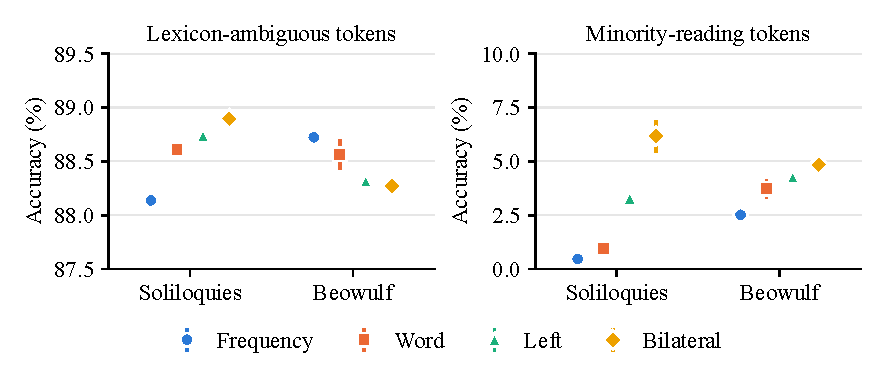
\includegraphics[width=15cm]{generated/fig_accuracy.pdf}
\caption{Accuracy on lexicon-ambiguous and minority-reading tokens (WikiPron run). Error bars: standard deviation
over seeds. The two panels use different y-axis ranges; exact values are in Table~\ref{tab:main}.}
\label{fig:acc}
\end{figure}

\paragraph{Context.} On the \textit{Soliloquies}, all three models beat the frequency baseline (word fixes \NWSolAFW{}
of the baseline's errors and makes \NWSolBFW{} new ones, $p=\NWSolPFW$). The gain comes from the word model's spelling
features, which generalise to candidates known only from WikiPron: adding context does not improve on the word
model (word vs.\ left $p=\NWSolPWL$, word vs.\ bilateral $p=\NWSolPWB$). On \textit{Beowulf}, no model beats the
baseline ($p\geq\NWBeoMinP$ for every comparison with it), and context is significantly \emph{worse} than the word
model (left fixes \NWBeoAWL{} of the word model's errors but makes \NWBeoBWL{} new ones, $p=\NWBeoPWL$; bilateral:
\NWBeoAWB{} against \NWBeoBWB, $p=\NWBeoPWB$). The gains from context are small everywhere and significant nowhere; the largest is on minority readings
(\NWSolMinWord\% to \NWSolMinBil\% on prose, not tested separately), still far below what the oracle shows is
possible.

\paragraph{Coverage.} Table~\ref{tab:abl} repeats the experiment with training forms as the only candidates.
WikiPron raises overall accuracy by \NSolGain{} points on prose and \NBeoGain{} points on \textit{Beowulf} for the
baseline, and by a similar amount for the models (\NBeoGainLeft--\NBeoGainWord{} points on \textit{Beowulf}). Without
it, \NBeoUnknown\% of \textit{Beowulf} tokens are words never seen in training, and for \NBeoNoCandTrue\% the
gold pattern is not a candidate at all. This is the largest effect in the
study. Without WikiPron, no model differs significantly from the baseline on either test set.

\begin{table}[h]
\centering
\caption{Dictionary ablation: accuracy (\%) with training-only candidates and with WikiPron added.}
\label{tab:abl}
\begin{tabular}{@{}llrrrr@{}}
\toprule
 & & \multicolumn{2}{c}{Training-only} & \multicolumn{2}{c}{+ WikiPron} \\
\cmidrule(lr){3-4}\cmidrule(l){5-6}
Test & System & All & Lex.-amb. & All & Lex.-amb. \\
\midrule
Soliloquies & Frequency & 87.23 & 88.25 & 88.69 & 88.06 \\
Soliloquies & Bilateral & 87.37 & 88.64 & 88.95 & 88.74 \\
Soliloquies & Oracle & 92.08 & 99.91 & 94.08 & 99.92 \\
\addlinespace
Beowulf & Frequency & 82.75 & 91.14 & 89.44 & 88.72 \\
Beowulf & Bilateral & 82.76 & 91.15 & 89.34 & 88.36 \\
Beowulf & Oracle & 85.32 & 100.00 & 92.73 & 100.00 \\

\bottomrule
\end{tabular}

\end{table}

\paragraph{Editors.} Harrison \& Sharp and Wyatt align on \NWAgrAligned{} tokens and agree on \NWAgrAll\% of them
(Cohen's $\kappa=\NWAgrAllK$ \cite{cohen1960}). On the \NWAgrAmbN{} lexicon-ambiguous aligned tokens they agree on
\NWAgrAmb\% ($\kappa=\NWAgrAmbK$). This is a human reference, not a strict upper bound, since our gold standard is a
third editor. Still, the best system on \textit{Beowulf} ambiguous tokens (\NWBeoLexWord\%) is \NEditorGap{} points
below the level at which two experts agree.

\section{Error analysis}
Table~\ref{tab:words} shows frequent ambiguous words in the \textit{Soliloquies} and how the training editions
mark them. Errors concentrate in a few function words whose marking differs between editions. \textit{ge} is long
in Zupitza (short/long \NGeZup) and Matthew (\NGeMat) but short in the \textit{Soliloquies} (\NGeSol): Matthew's
\textit{gē} is mostly the pronoun `ye', while the \textit{Soliloquies} mostly use the conjunction \textit{ge}
`and', so this difference is lexical and driven by genre. \textit{se} is long in Bright and Matthew but mostly
short in Zupitza, Sweet and the test text, which is editorial habit. \textit{þe} and \textit{ne} are grammatical:
the relative particle vs.\ the pronoun `thee', and `not' vs.\ `nor'. These category labels are preliminary; two
annotators and Cohen's $\kappa$ are needed to confirm them, and leave-one-editor-out training to test whether
mixed conventions cause the errors.

\begin{table}[h]
\centering
\caption{Frequent lexicon-ambiguous words in the \textit{Soliloquies} (training-only run): token count, gold
short/long counts, accuracy (\%) of frequency and bilateral (seed~1), and short/long counts in three training editions.}
\label{tab:words}
\begin{tabular}{@{}lrrrrrrr@{}}
\toprule
Word & \textit{n} & Gold s/l & Freq. & Bil. & Zupitza s/l & Matthew s/l & Bright s/l \\
\midrule
\textit{þæt} & 679 & 675/4 & 99.4 & 99.4 & 343/0 & 426/0 & 1001/1 \\
\textit{þe} & 567 & 327/240 & 57.7 & 64.0 & 309/50 & 364/126 & 574/128 \\
\textit{þu} & 491 & 1/490 & 99.8 & 99.8 & 0/229 & 2/151 & 0/201 \\
\textit{ne} & 348 & 268/80 & 77.0 & 76.4 & 100/29 & 260/48 & 312/136 \\
\textit{to} & 191 & 32/159 & 83.2 & 83.2 & 1/237 & 14/313 & 24/619 \\
\textit{se} & 72 & 48/24 & 33.3 & 33.3 & 199/62 & 3/330 & 6/465 \\
\textit{ge} & 64 & 61/3 & 4.7 & 28.1 & 0/128 & 2/252 & 84/70 \\
\bottomrule
\end{tabular}

\end{table}

Two sentences show what the context models miss:

\begin{quote}
\textit{Ic clypie tō þē, Drihten, þū þe æall geworhtest, \dots} `I call to thee, Lord, thou who madest all \dots'\\
\textit{Tō þē ic clypige, þe nēfre nān yfel ne worhtest, ac ǣlc gōd weorc worhtest.} `To thee I call, who never
wrought any evil, but wrought every good work.'
\end{quote}

\noindent In both, every system predicts short \textit{þe} in \textit{tō þē}, where the gold is the pronoun
\textit{þē}, although the left model has the preposition \textit{tō} directly before the word. In fact the
models almost never output \textit{þē}: the left model predicts the long form for \NTheLongLeft{} of the
\NTheTokens{} \textit{þe} tokens in the test text, and the left and bilateral models both miss \NToTheMissed{} of the
\NToTheN{} long \textit{þē} that follow \textit{tō}. A linear model over word identities does not learn that a
preposition before \textit{þe} signals the pronoun, which motivates an encoder that reads the whole sentence. The same text also shows
a transcription slip (\textit{þū pe} for \textit{þū þe}), a reminder that the source transcriptions are not error-free.

\section{Deviations, limitations and future work}
\textbf{Deviations from the proposal.} We used logistic classifiers instead of a fine-tuned ByT5 encoder, WikiPron
instead of the Clark Hall and Bosworth--Toller dictionaries, and did not carry out the CharsiuG2P error analysis.
The Gospel of John was not used as a development set because no hyperparameters were tuned.
\textbf{Limitations.} The WikiPron alignment is heuristic, McNemar tests treat tokens as independent although they
cluster in sentences, and all labels are editorial decisions rather than recorded pronunciation.
\textbf{Future work.} A ByT5 encoder over full sentences, a comparison with CharsiuG2P, historical dictionaries,
two-annotator ambiguity classes, and leave-one-editor-out training.
\textbf{Conclusion.} In our experiments, dictionary coverage limits Old English macron restoration far more than a
two-word context window does; differences in how editions mark frequent function words are a likely further
limit, which a leave-one-editor-out study should test.

\begin{thebibliography}{9}
\bibitem{cohen1960} J.~Cohen. A coefficient of agreement for nominal scales. \textit{Educational and Psychological
Measurement}, 20(1):37--46, 1960.
\bibitem{klaeber1922} F.~Klaeber, editor. \textit{Beowulf and the Fight at Finnsburg}. D.~C.~Heath, Boston, 1922.
\bibitem{lee2020} J.~L.~Lee, L.~F.~E.~Ashby, M.~E.~Garza, Y.~Lee-Sikka, S.~Miller, A.~Wong, A.~D.~McCarthy and
K.~Gorman. Massively multilingual pronunciation modeling with WikiPron. In \textit{Proceedings of LREC 2020},
pages 4223--4228, 2020.
\bibitem{mcnemar1947} Q.~McNemar. Note on the sampling error of the difference between correlated proportions or
percentages. \textit{Psychometrika}, 12(2):153--157, 1947.
\bibitem{pedregosa2011} F.~Pedregosa et al. Scikit-learn: Machine learning in Python. \textit{Journal of Machine
Learning Research}, 12:2825--2830, 2011.
\bibitem{tauber} J.~Tauber. \textit{old-english-texts}, \texttt{beowulf/raw-data/brunetti-length.txt}.
\url{https://github.com/old-english-learner-texts/old-english-texts}. CC BY-SA 4.0.
\bibitem{winge2015} J.~Winge. \textit{Automatic annotation of Latin vowel length}. Bachelor's thesis, Uppsala
University, 2015.
\bibitem{yarowsky1994} D.~Yarowsky. Decision lists for lexical ambiguity resolution: Application to accent
restoration in Spanish and French. In \textit{Proceedings of ACL 1994}, pages 88--95, 1994.
\bibitem{zhu2022} J.~Zhu, C.~Zhang and D.~Jurgens. ByT5 model for massively multilingual grapheme-to-phoneme
conversion. In \textit{Proceedings of Interspeech 2022}, 2022.
\bibitem{editions} Project Gutenberg, \url{https://www.gutenberg.org/ebooks/}: 9701 (Harrison \& Sharp), 45861 (Zupitza),
34316 (Sweet), 14529 (Cook \& Pitman). Wikisource, \url{https://en.wikisource.org/wiki/}: \nolinkurl{Beowulf_(Wyatt)},
\nolinkurl{Bright's_Anglo-Saxon_Reader}, \nolinkurl{Evangelium_Secundum_Mattheum},
\nolinkurl{King_Alfred's_Old_English_Version_of_St._Augustine's_Soliloquies} (Hargrove).
\end{thebibliography}
\end{document}
